%%%%%%%%%%%%%%%%%%%%%%%%%%%%%%%%%%%%%%%%%%%%%%%%%%%%%%%%%%%%%%%%%%%%%
%% This is a (brief) model paper using the achemso class
%% The document class accepts keyval options, which should include
%% the target journal and optionally the manuscript type.
%%%%%%%%%%%%%%%%%%%%%%%%%%%%%%%%%%%%%%%%%%%%%%%%%%%%%%%%%%%%%%%%%%%%%
\documentclass[journal=jctcce,manuscript=article]{achemso}
% \setkeys{acs}{articletitle=false}

%%%%%%%%%%%%%%%%%%%%%%%%%%%%%%%%%%%%%%%%%%%%%%%%%%%%%%%%%%%%%%%%%%%%%
%% Place any additional packages needed here.  Only include packages
%% which are essential, to avoid problems later. Do NOT use any
%% packages which require e-TeX (for example etoolbox): the e-TeX
%% extensions are not currently available on the ACS conversion
%% servers.
%%%%%%%%%%%%%%%%%%%%%%%%%%%%%%%%%%%%%%%%%%%%%%%%%%%%%%%%%%%%%%%%%%%%%
\usepackage[version=3]{mhchem} % Formula subscripts using \ce{}
\usepackage{chemnum}
\usepackage{multirow}
\usepackage{textgreek}
\usepackage{textcomp}
\usepackage{setspace}
\usepackage{afterpage}
\usepackage{caption}
\usepackage{floatrow}
\usepackage{gensymb}
\usepackage{mathtools}

\usepackage{csquotes}


\usepackage{epigraph}
\renewcommand{\epigraphsize}{\small}
\renewcommand{\textflush}{flushright} \renewcommand{\sourceflush}{flushright}

\let\originalepigraph\epigraph 
\renewcommand\epigraph[2]{\originalepigraph{\textit{#1}}{\textsc{#2}}}
\setlength{\epigraphwidth}{0.5\textwidth}

\renewcommand{\textflush}{flushright} \renewcommand{\sourceflush}{flushright}




\usepackage[most]{tcolorbox}


\captionsetup{justification=raggedright,singlelinecheck=false}
\usepackage[labelfont=bf]{caption}
\usepackage{makecell}

\usepackage{dblfloatfix}
\usepackage{framed}

\usepackage{natbib}
\usepackage[acroymn]{glossaries}
\usepackage{tabularx} % for 'tabularx' environment
\usepackage{array}

\usepackage{acro}

\acsetup{hyperref=true}

\usepackage{enumitem}

\usepackage{multicol}
\usepackage{graphicx}
\usepackage{subcaption}

% glossary
\usepackage{hyperref}


\hypersetup{
    colorlinks,
    citecolor=black,
    filecolor=black,
    linkcolor=black,
    urlcolor=black
}



%%%%%%%%%%%%%%%%%%%%%%%%%%%%%%%%%%%%%%%%%%%%%%%%%%%%%%%%%%%%%%%%%%%%%
%% If issues arise when submitting your manuscript, you may want to
%% un-comment the next line.  This provides information on the
%% version of every file you have used.
%%%%%%%%%%%%%%%%%%%%%%%%%%%%%%%%%%%%%%%%%%%%%%%%%%%%%%%%%%%%%%%%%%%%%
%%\listfiles

%%%%%%%%%%%%%%%%%%%%%%%%%%%%%%%%%%%%%%%%%%%%%%%%%%%%%%%%%%%%%%%%%%%%%
%% Place any additional macros here.  Please use \newcommand* where
%% possible, and avoid layout-changing macros (which are not used
%% when typesetting).
%%%%%%%%%%%%%%%%%%%%%%%%%%%%%%%%%%%%%%%%%%%%%%%%%%%%%%%%%%%%%%%%%%%%%
\newcommand*\mycommand[1]{\texttt{\emph{#1}}}

%%%%%%%%%%%%%%%%%%%%%%%%%%%%%%%%%%%%%%%%%%%%%%%%%%%%%%%%%%%%%%%%%%%%%
%% Meta-data block
%% ---------------
%% Each author should be given as a separate \author command.
%%
%% Corresponding authors should have an e-mail given after the author
%% name as an \email command. Phone and fax numbers can be given
%% using \phone and \fax, respectively; this information is optional.
%%
%% The affiliation of authors is given after the authors; each
%% \affiliation command applies to all preceding authors not already
%% assigned an affiliation.
%%
%% The affiliation takes an option argument for the short name.  This
%% will typically be something like "University of Somewhere".
%%
%% The \altaffiliation macro should be used for new address, etc.
%% On the other hand, \alsoaffiliation is used on a per author basis
%% when authors are associated with multiple institutions.
%%%%%%%%%%%%%%%%%%%%%%%%%%%%%%%%%%%%%%%%%%%%%%%%%%%%%%%%%%%%%%%%%%%%%
\author{Eric D. Boittier}
\email{eric.boittier@uqconnect.edu.au}
\affiliation[UQ]{The University of Queendland, St Lucia, Queensland, Australia}

\author{\linebreak Supervisors: A/Professor Vito Ferro}
\affiliation[UQ]{The University of Queendland, St Lucia, Queensland, Australia}

\author{Dr Neha Gandhi}
\affiliation[QUT]{Queensland University of Technology, Gardens Point, Queensland, Australia}


%%%%%%%%%%%%%%%%%%%%%%%%%%%%%%%%%%%%%%%%%%%%%%%%%%%%%%%%%%%%%%%%%%%%%
%% The document title should be given as usual. Some journals require
%% a running title from the author: this should be supplied as an
%% optional argument to \title.
%%%%%%%%%%%%%%%%%%%%%%%%%%%%%%%%%%%%%%%%%%%%%%%%%%%%%%%%%%%%%%%%%%%%%
\title[Honours]
  {Parameterisation of ``VinaCarb" for improved docking of heparin/heparan sulfate  \linebreak \large Research Proposal}

%%%%%%%%%%%%%%%%%%%%%%%%%%%%%%%%%%%%%%%%%%%%%%%%%%%%%%%%%%%%%%%%%%%%%
%% Some journals require a list of abbreviations or keywords to be
%% supplied. These should be set up here, and will be printed after
%% the title and author information, if needed.
%%%%%%%%%%%%%%%%%%%%%%%%%%%%%%%%%%%%%%%%%%%%%%%%%%%%%%%%%%%%%%%%%%%%%
% \abbreviations{IR,NMR,UV}
% \keywords{American Chemical Society}

\DeclareAcronym{Ido}{
    short = IdoA ,
    long = {\small L}-iduronic acid
}

\DeclareAcronym{Glc}{
    short = Glc ,
    long = {\small D}-glucose
}

\DeclareAcronym{AD4}{
    short = AD4 ,
    long = AutoDock 4
}

\DeclareAcronym{DFT}{
    short = DFT ,
    long = Desnity Functional Theory
}

\DeclareAcronym{Gal}{
    short = Gal ,
    long = {\small D}-galactose
}

\DeclareAcronym{DFT}{
    short = DFT ,
    long = density functional theory
}

\DeclareAcronym{GlcN}{
    short = GlcN ,
    long = {\small D}-glucosamine
}

\DeclareAcronym{PDB}{
    short = PDB,
    long = Protein Data Bank
}

\DeclareAcronym{MC}{
    short = MC,
    long = Monte Carlo
}

\DeclareAcronym{GS}{
    short = GS,
    long = genetic search
}

% \DeclareAcronym{GalA}{
%     short = GalA ,
%     long = {\small D}-galacturonic acid
% }

\DeclareAcronym{GlcA}{
    short = GlcA ,
    long = {\small D}-glucuronic acid
}

\DeclareAcronym{GalN}{
    short = GalN ,
    long = {\small D}-galactosamine
}

\DeclareAcronym{GlcNAc}{
    short = GlcNAc ,
    long = N-acetyl-{\small D}-glucosamine
}

\DeclareAcronym{PG}{
    short = PG ,
    long = proteoglycan
}

\DeclareAcronym{CHI}{
    short = CHI ,
    long = CarboHydrate Intrinsic
}

\DeclareAcronym{ECM}{
    short = ECM ,
    long = extracellular matrix
}

\DeclareAcronym{GAG}{
    short = GAG ,
    long = glycosaminoglycan
}

\DeclareAcronym{Hep}{
    short = Hep ,
    long = heparin
}
\DeclareAcronym{HS}{
    short = HS ,
    long = heparan sulfate
}
\DeclareAcronym{HA}{
    short = HA ,
    long = hyaluronic acid
}
\DeclareAcronym{CS}{
    short = CS,
    long = chondroitin sulfate
}
\DeclareAcronym{KS}{
    short = KS,
    long = keteran sulfate
}
\DeclareAcronym{DS}{
    short = DS,
    long = dermatin sulfate
}


\DeclareAcronym{DoS}{
    short = DoS,
    long = degrees of sulfation
}

\DeclareAcronym{SNFG}{
    short = SNFG, 
    long = structural nomenclature for glycans
}


\DeclareAcronym{APP}{
    short = APP,
    long = amyloid precursor protein
}
\DeclareAcronym{Al}{
    short = APP,
    long = amyloid precursor protein
}
\DeclareAcronym{QM}{
    short = QM,
    long = quantum mechanics
}
\DeclareAcronym{MD}{
    short = MD,
    long = molecular dynamics
}

\DeclareAcronym{FGF1}{
    short = FGF1,
    long = fibroblast growth factor 1
}
\DeclareAcronym{FGF2}{
    short = FGF2,
    long = fibroblast growth factor 2
}
\DeclareAcronym{FGF}{
    short = FGF,
    long = fibroblast growth factor 
}
\DeclareAcronym{AT3}{
    short = ATIII,
    long = \textalpha-antithrombin III
}

\DeclareAcronym{RMSD}{
    short = RMSD,
    long = root mean square deviation
}
\DeclareAcronym{PRMSD}{
    short = PRMSD,
    long = pose root mean square deviation
}

\DeclareAcronym{RBD}{
    short = RBD,
    long = rigid body docking
}

\DeclareAcronym{ADV}{
    short = ADV,
    long = AutoDock Vina
}

\DeclareAcronym{THP}{
    short = THP,
    long = tetrahydropyran
}



\DeclareAcronym{SAR}{
    short = SAR,
    long = structure activity relationship
}

\newcommand{\squeezeup}{\vspace{-2.5mm}}


\begin{document}
\pagenumbering{gobble}
\renewcommand{\thefootnote}{\fnsymbol{footnote}}
\pagenumbering{roman} 

%%%%%%%%%%%%%%%%%%%%%%%%%%%%%%%%%%%%%%%%%%%%%%%%%%%%%%%%%%%%%%%%%%%%%
%% The manuscript does not need to include \maketitle, which is
%% executed automatically.  The document should begin with an
%% abstract, if appropriate.  If one is given and should not be, the
%% contents will be gobbled.
%%%%%%%%%%%%%%%%%%%%%%%%%%%%%%%%%%%%%%%%%%%%%%%%%%%%%%%%%%%%%%%%%%%%%
{\setstretch{1.5} 
\renewcommand{\contentsname}{Table of Contents}

\renewcommand{\thesubfigure}{\Alph{subfigure}}

\newpage
\tableofcontents
\newpage
\listoffigures
\listoftables
\newpage
\begin{multicols}{2}
{\setstretch{1}
\printacronyms[name={Abbreviations}, list-style={table}]
}
\end{multicols}

%%%%%%%%%%%%%%%%%%%%%%%%%%%%%%%%%%%%%%%%%%%%%%%%%%%%%%%%%%%%%%%%%%%%%
%% Start the main part of the manuscript here.
%%%%%%%%%%%%%%%%%%%%%%%%%%%%%%%%%%%%%%%%%%%%%%%%%%%%%%%%%%%%%%%%%%%%%
\pagebreak
\pagenumbering{arabic} 
\section{Background}

\subsection{Heparin and heparan sulfate} 

\setlength{\textfloatsep}{0.5cm}

\begin{figure}[bl!]

    {\renewcommand{\arraystretch}{1.5}
    \setlength{\tabcolsep}{0.3cm}
    
    
    
    \begin{tabular}{p{1.4cm}p{0.45\textwidth}p{0.4\textwidth}}
        & \textbf{~~~~~~~Heparin} & \textbf{~~~~~Heparan sulfate} 
    \end{tabular}
    
    {\centering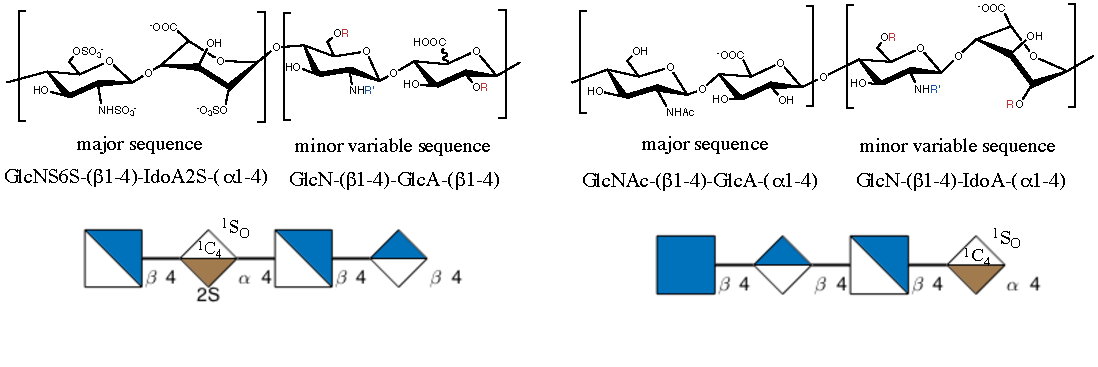
\includegraphics[width=17cm]{HeparinHeparanSulfate.pdf}}
    
    \begin{tabular}{p{1.9cm}|p{0.4\textwidth}p{0.1mm}p{0.36\textwidth}}
   
    
      Location:  & \makecell{\hspace{-1.8cm}\textbullet~  Intracellular compent of \\ \hspace{-1cm} mast cells, esp. lungs, skin.} 
      & &\makecell{\textbullet~ Ubiquitious component of cell \\ \hspace{-1.05cm}surfaces in the ECM.} \\ 
    \renewcommand{\arraystretch}{1}
      Mass: & \textbullet~ 10-12 kDa & & \textbullet~ 10--70 kDa \\
      \renewcommand{\arraystretch}{1.3}
      DoS:  &  \textbullet~ 1.8--2.4 & &  \textbullet~ 0.8--1.8 \\
      GlcA:IdoA & \textbullet~ 1:9 & & \textbullet~ 8:2
    \end{tabular}}
    \caption{The differences between heparin/heparan sulfate, including the chemical structure (R = SO$_{3}^{-}$ or H, R' = SO$_{3}^{-}$ or Ac), the Symbol Nomenclature for Glycans (SNFG) representation, biological origin, mass, degree of solvation (DoS) and ratios between glucuronic acid to glucosamine residues.}
    
    %\cite{Varki2009SymbolRepresentation} 
    
    \label{fig:HepHS}
\end{figure}

On the surface of all eukariotic cells, highly sulfated complex oligosaccharides known as \acp{GAG} act as emissaries for the reception and modulation of a wide range of proteins. \cite{Capila2002Heparin-proteinInteractions., Gandhi2008TheProteins, Casu2005StructureHeparin, Imberty2007StructuralInteractions}
These sugars affect normal physiological processes, such as blood coagulation and neuronal development, and serious pathophysiological disorders, such as cancer and Alzhiemer's disease. \cite{Nieto2011ConformationalReceptor, Hu2012DivergentInteraction, Thompson1994EnergeticDomain, Guimond1999FibroblastSaccharides., Faham1996HeparinFactor, Li2004StructureHeparin} 
\Ac{Hep} and the closely related \ac{HS} are members of the \ac{GAG} family. \Ac{Hep} possesses the highest negative charge density in all of nature. \cite{Capila2002Heparin-proteinInteractions., Gandhi2008TheProteins}
\ac{Hep} and \ac{HS} bind to \ac{GAG} specific receptors on proteins such as chemokines, cytokines, growth factors, morphogens, enzymes and adhesion molecules.\cite{Murphy2007StructuralHeparin, Iozzo2001HeparanArena, Kreuger2006InteractionsSpecificity, Kowitsch2018MedicalReview} 
In the clinic, \ac{Hep} is a widely used anticoagulant drug to treat patients with cardiovascular  disorders.\cite{Liu2014ChemoenzymaticHeparin.}

\subsubsection{Structure}\label{structure}
\ac{Hep} and \ac{HS}, like all \acp{GAG}, are comprised of repeating disaccharides containing uronic acid residues (\ac{Ido} or its C5 epimer, \ac{GlcA}, which are \textalpha~or  \textbeta 1\textrightarrow4-linked, respectively) paired with \textalpha 1\textrightarrow4-linked \ac{GlcN} residues (Figure \ref{fig:HepHS}). \cite{Capila2002Heparin-proteinInteractions., Gandhi2008TheProteins, Casu2005StructureHeparin}
\acp{GAG} exhibit various sulfation patterns and \ac{DoS} (i.e. the number of sulfonate groups per disaccharide). These structural features are a product of around 26 proteins involved in \ac{GAG} biosynthesis in the golgi apparatus.\cite{SoaresdaCosta2017SulfationDisorders, Varki2009BiologicalGlycans}
The structural encoding ability of \acp{GAG} rivals that of DNA, RNA and proteins.\cite{Gama2006SulfationActivity} 
The amino sugar can be sulfated at C4, C6, the unsubstituted nitrogen or C3 (rare), and the uronic acid residue can be substituted at C2 or C3 -- leading to \textgreater1,000,000 possible substitution patterns for a \ac{GAG} octasaccharide.\cite{Gandhi2008TheProteins, SoaresdaCosta2017SulfationDisorders,Gama2006SulfationActivity} 
\ac{HS} occurs in many cell types, while heparin is isolated exclusively from mast cells.\cite{Liu2014ChemoenzymaticHeparin., Gandhi2008TheProteins}
Here, both sugars are found attached to the surface of \acp{PG}, where they are can facilitate recognition and cell signalling. \cite{Capila2002Heparin-proteinInteractions., Gandhi2008TheProteins, Casu2005StructureHeparin}
While \ac{Hep} and \ac{HS} are comprised of similar disaccharide building blocks, their \ac{DoS} and ratios between \ac{GlcA} and \ac{Ido} differ. \cite{Capila2002Heparin-proteinInteractions., Gandhi2008TheProteins, Casu2005StructureHeparin}
\ac{Hep} has higher sulfation levels than HS (\ac{DoS} 2.6 vs 0.6, respectively). \cite{Nahain2018HeparinActivity, Avci2003SyntheticProperties, }
Upregulation of \ac{Ido} also varies; around 9 in 10 of the disaccharide units in \ac{Hep} contain \ac{Ido}, while only 2 in 10 \ac{HS} disaccharide units contain \ac{Ido}. \cite{Capila2002Heparin-proteinInteractions., Gandhi2008TheProteins, Casu2005StructureHeparin}

\subsubsection*{~~~~~~~~~Ring conformations}

Flexible ring conformations of \ac{GAG} components add further structural complexity to the oligosaccharide and are reasoned to have biological relevance during \ac{GAG}--protein interactions.\cite{Sattelle2013DoesHeparanome} 
Although \ac{GlcA} and \ac{GlcN} remain in the standard $^{4}C_{1}$ conformation, the exceptional plasticity of \ac{Ido} ring conformations is unique among sugars, and is dependent on its position in the chain, ionic conditions and sulfation pattern.\cite{Capila2002Heparin-proteinInteractions., vanBoeckel1987ConformationalAcid}
At the reducing end, \ac{Ido} has been characterized as existing in an equilibrium between $^{4}C_{1}$, $^{1}C_{4}$ and $^{2}S_{O}$, using $^{1}$H NMR spectroscopy (Figure \ref{fig:ido_confs} A).\cite{Ferro1986EvidenceStudies, vanBoeckel1987ConformationalAcid} 
\begin{figure}[tl!]
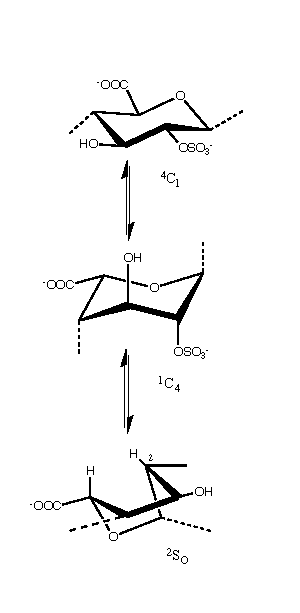
\includegraphics[width=12cm]{ido_confs.pdf}
\caption{\textbf{(A)} Conformational equilibrium of iduronic acid in solution and bound to the protein. \textbf{(B)} The diversity of iduronic ring conformations }
\label{fig:ido_confs}
\end{figure}
When \ac{Ido} is inside the chain, the equilibrium favors the $^{1}C_{4}$ and $^{2}S_{O}$ conformations exclusively, due to interactions with the 1\textrightarrow4-linked neighbouring sugar.\cite{vanBoeckel1987ConformationalAcid} 
When \ac{Ido} is sulfated at the C2 position, the $^{2}S_{O}$ conformer may become more prominent to minimize unfavorable 1,3 diaxial interactions in the $^{1}C_{4}$ structure.\cite{Hsieh2016UncoveringSulphateb} However, the barrier for interconversion between the two conformers is low and has little effect on the overall conformation of the oligosaccharide, allowing \ac{Ido} to adopt poses suited for specific interactions with proteins. \cite{Capila2002Heparin-proteinInteractions., Woods2018PredictingComplexes} 
In the case of the \ac{Hep} and \ac{FGF2} complex, two \ac{Ido} residues are poised in $^{1}C_{4}$ and $^{2}S_{O}$ conformations respectively (Figure \ref{fig:ido_confs} B, \ac{PDB} entry 1I8Q),).\cite{Faham1996HeparinFactor} 
Ring flipping, which is believed to occur on the \textmu s timescale based on \ac{MD} simulations (\ac{MD} is covered in Section 
\ref{MD}).\cite{Sattelle2012DependenceIdopyranosides} 
Ring flipping has been a proposed as mechanism for selective binding/unbinding.\cite{Faham1996HeparinFactor} 

{\renewcommand{\arraystretch}{1.5}
\setlength{\tabcolsep}{0.3cm}

\begin{table}[bl!]
    \hspace{}
    \begin{tabular}{p{2cm}p{5.5cm}p{7.5cm}}
        \hline
        Technique & Characterization & Disadvantages  \\
        \hline 
        \makecell[tl]{X-ray \\ crystall--\\ography} & 3D structure of ligand--protein complex in a single low energy conformation & \makecell[tl]{\textbullet $ $ Often errors in residue structures/names\\ \textbullet $ $  Only identifies one conformation\\ \textbullet $ $  Poor resolution can lead to incorrect \\~~~structures\\ \textbullet $ $  Protons are not characterized } \\
        
        NMR & Time averaged angles, dihedrals and distance between protons, structural connectivity & 
        \makecell[tl]{\textbullet $ $ Time averaged structure cannot inform \\ \hspace{3mm} structural ensembles\\ \textbullet $ $  Innappropriate for long (\textgreater\textmu s) timescales \\ \textbullet $ $  Small error in coupling constants result \\ \hspace{3mm} in large structural uncertainty }\\ 
    
        \makecell[tl]{Molecular \\ dynamics} & Simulations of the structure of ligand--protein complexes over time & \makecell[tl]{\textbullet $ $ Relies on accurate forcefields and models \\ \textbullet $ $  Computationally expensive for long \\ \hspace{3mm} (\textgreater\textmu s) timescales}  \\
        \hline
        
    \end{tabular}
    \caption{Experimental and \textit{in silico} methods for characterisation of the 3D structure of glycosaminoglycans.}
    \label{tab:GAGprotein}
\end{table}
}
Standard NMR techniques struggle to discriminate between the exchange of even the most simple conformers on the \textmu s timescale - at best only 10\% of conformers are perceptible (See Table \ref{tab:GAGprotein}).\cite{Sattelle2011IsChair} 
Therefore \ac{MD} simulations are crucial to gain insite into these types of structural equilibria.\cite{Woods2018PredictingComplexes} 

\subsubsection*{~~~~~~~~~Glycosidic torsions: \textphi~and \textphi}

\begin{figure}[bl!]
    \centering
    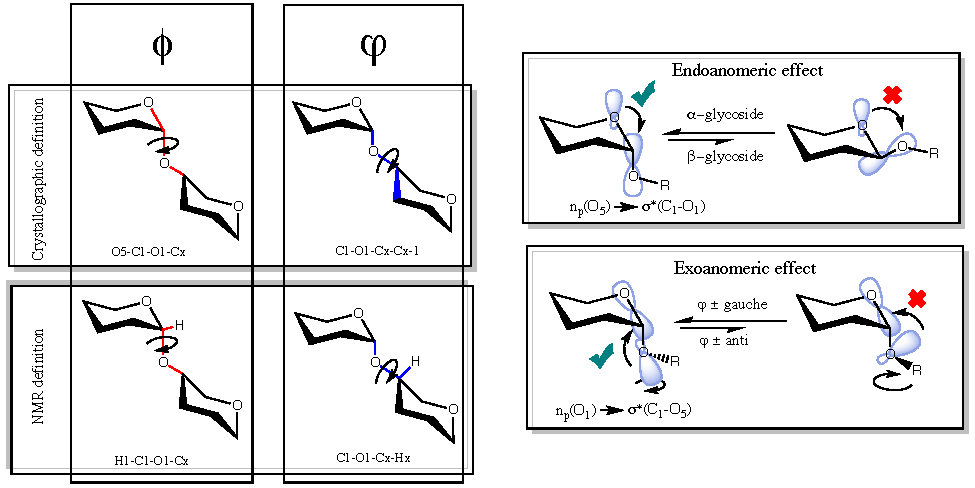
\includegraphics[width=14cm]{phi_psi_endo_exo.pdf}
    \caption{\textbf{(A)} The crystallographic and NMR definitions of the \textphi~ and \textpsi~ torsions of oligosaccharides. \textbf{(B)} The endoanomeric effect as an explanation for the increased stability of \textalpha~--glycosides. \textbf{(C)} The exoanomeric effect as an explanation for the preference of gauche conformations of \textpsi~ torsions. }
    \label{fig:phipsiendoexo}
\end{figure}

Oligosaccharides have two axis of free rotation, or torsions, around the glycosidic linkage, defined as \textphi~and \textpsi~(Figure \ref{fig:phipsiendoexo} A). When analysing data from crystallography, the dihedrals, \textphi~and \textpsi, may be defined using the atoms O5--C1--O1--CX and C1--O1--C$x$--C$(x-1)$, respectively. \cite{Nivedha2016Vina-Carb:Docking, Lutteke2005CarbohydratePDB.}
Alternatively, \textphi~and \textpsi~may be found using NMR observables (where the dihedrals are defined as H1--C1--O1--C$x$ and C1--O1--C$x$--H$x$, respectively). \cite{Hricovini2015SolutionAnalysis., Nivedha2016Vina-Carb:Docking, Pol-Fachin2008DepictionSolutions}
In general, the answer to ``how flexible are the glycosidic linkages inside an oligosaccharide?'' may differ depending on the chemist answering the question. 
To a protein crystollographer, the absence of secondary or tertiary structural elements may prompt them to classify these polymers as flexible. \cite{Woods1998TheMolecule}
However, a carbohydrate chemist familiar with NMR or crystallographic data, may disagree, since these dihedrals usually only deviate by at most 90\textdegree, when comparing disaccharide pairs that share simillar linkage geometries (i.e. \textalpha~and \textbeta~linkages to axial/equitorial substituents)).\cite{Clerc2018ASpace, Hricovini2015SolutionAnalysis}
This has been attributed to the exoanomeric effect (Figure \ref{fig:phipsiendoexo} C), where favorable orbital interactions between the non-bonding p-orbital of the oxygen participating in the glycosidic bond and the $\sigma^{*}$ orbital of the O5--C1 bond. \cite{Woods2018PredictingComplexes}
This interaction is analogous to the endoanomomeric effect (Figure \ref{fig:phipsiendoexo} B), where favorable orbital interactions between the non-bonding p-orbital of the ring oxygen and the $\sigma^{*}$ orbital of the C1--O1 bond lead to the preference for \textalpha-glycosides. \cite{Varki2009BiologicalGlycans}

\subsubsection{Protein interactions}

\subsubsection*{~~~~~~~~~Electrostatic interactions}


\ac{Hep} and \ac{HS} bind to the surface of proteins due to their size and hydrophillic nature. At physiological pH, all carboxylic acid and sulfate groups are deprotonated.\cite{Capila2002Heparin-proteinInteractions., Gandhi2008TheProteins, Casu2005StructureHeparin, Imberty2007StructuralInteractions}
These negatively charged moieties recognize shallow pocket regions of positive charge on the protein surface through electrostatic interactions.\cite{Capila2002Heparin-proteinInteractions., Gandhi2008TheProteins, Casu2005StructureHeparin, Imberty2007StructuralInteractions}
Electrostatic interactions are nondirectional and operate over longer distance than those that rely on hydrogen bond or van der Waals forces. Coulombic forces have a $ r^{-1}$  relationship (where $r$ is the distance between two ions), whereas vander Waals forces have a  $ r^{-3}$ to  $ r^{-6}$ dependence. \cite{Sankaranarayanan2014TowardProteins, Kirschner2008GLYCAM06:Carbohydrates} 
Generally, hydrogen bond distances are between 2 - 4 \AA, whereas the cutoff for charged interactions can be as high as 8 \AA. \cite{FerreiradeFreitas2017APDB}
For this reason, electrostatic interactions are generally nonspecific to the binding pose geometry.\cite{Sarkar2016EstimatingInteraction.}
Residues associated with these positively charged GAG binding surfaces are predominantly Arg and Lys, but His is also involved in some complexes. Arg binds with 2.5 times more affinity than Lys. \cite{Capila2002Heparin-proteinInteractions.}
The guanidino group in Arg displays stronger electrostatic interactions with sulfate groups, and more stable hydrogen boding \cite{Hileman1998Glycosaminoglycan-proteinProteins}. 
Due the high repulsive energy associated with multiple negatively charged groups, cations (such as Na$^{+}$) bind to minimize these unfavourable forces (although this process is entropically unfavourable)  \cite{Hileman1998Glycosaminoglycan-proteinProteins}
To bind to a protein, cations coordinated to the \ac{GAG} must be displaced. \cite{}
Simillarly, any anions coordinated to Lys, Arg or His must also be displaced. This is also known as the ``polyelectrolyte effect'' and can be considered a screening effect, since the competing GAG--protein interactions must be strong enough to displace these ions.\cite{CardinMolecularInteractions.}
As expected, an increase in the concentration of salt reduces ligand binding. \cite{Capila2002Heparin-proteinInteractions., Gandhi2008TheProteins} 
\acp{GAG} share features in common with DNA; both are linear, negatively charge polymers. 
In the case of DNA and heparin, this has been shown by sodium--23 NMR and isothermal titration calorimetry, respectively\cite{Anderson1978Sodium-23Interactions., Thompson1994EnergeticDomain}.  
While charged interactions have been highlighted as important for recognition of the binding site\cite{Samsonov2016ComputationalComplexes}, these interactions are nonspecific. Almost any protein surface containing positive charge will recognize a sulfated GAG chain.\cite{CardinMolecularInteractions.}

\begin{figure}[bl!]
    \centering
    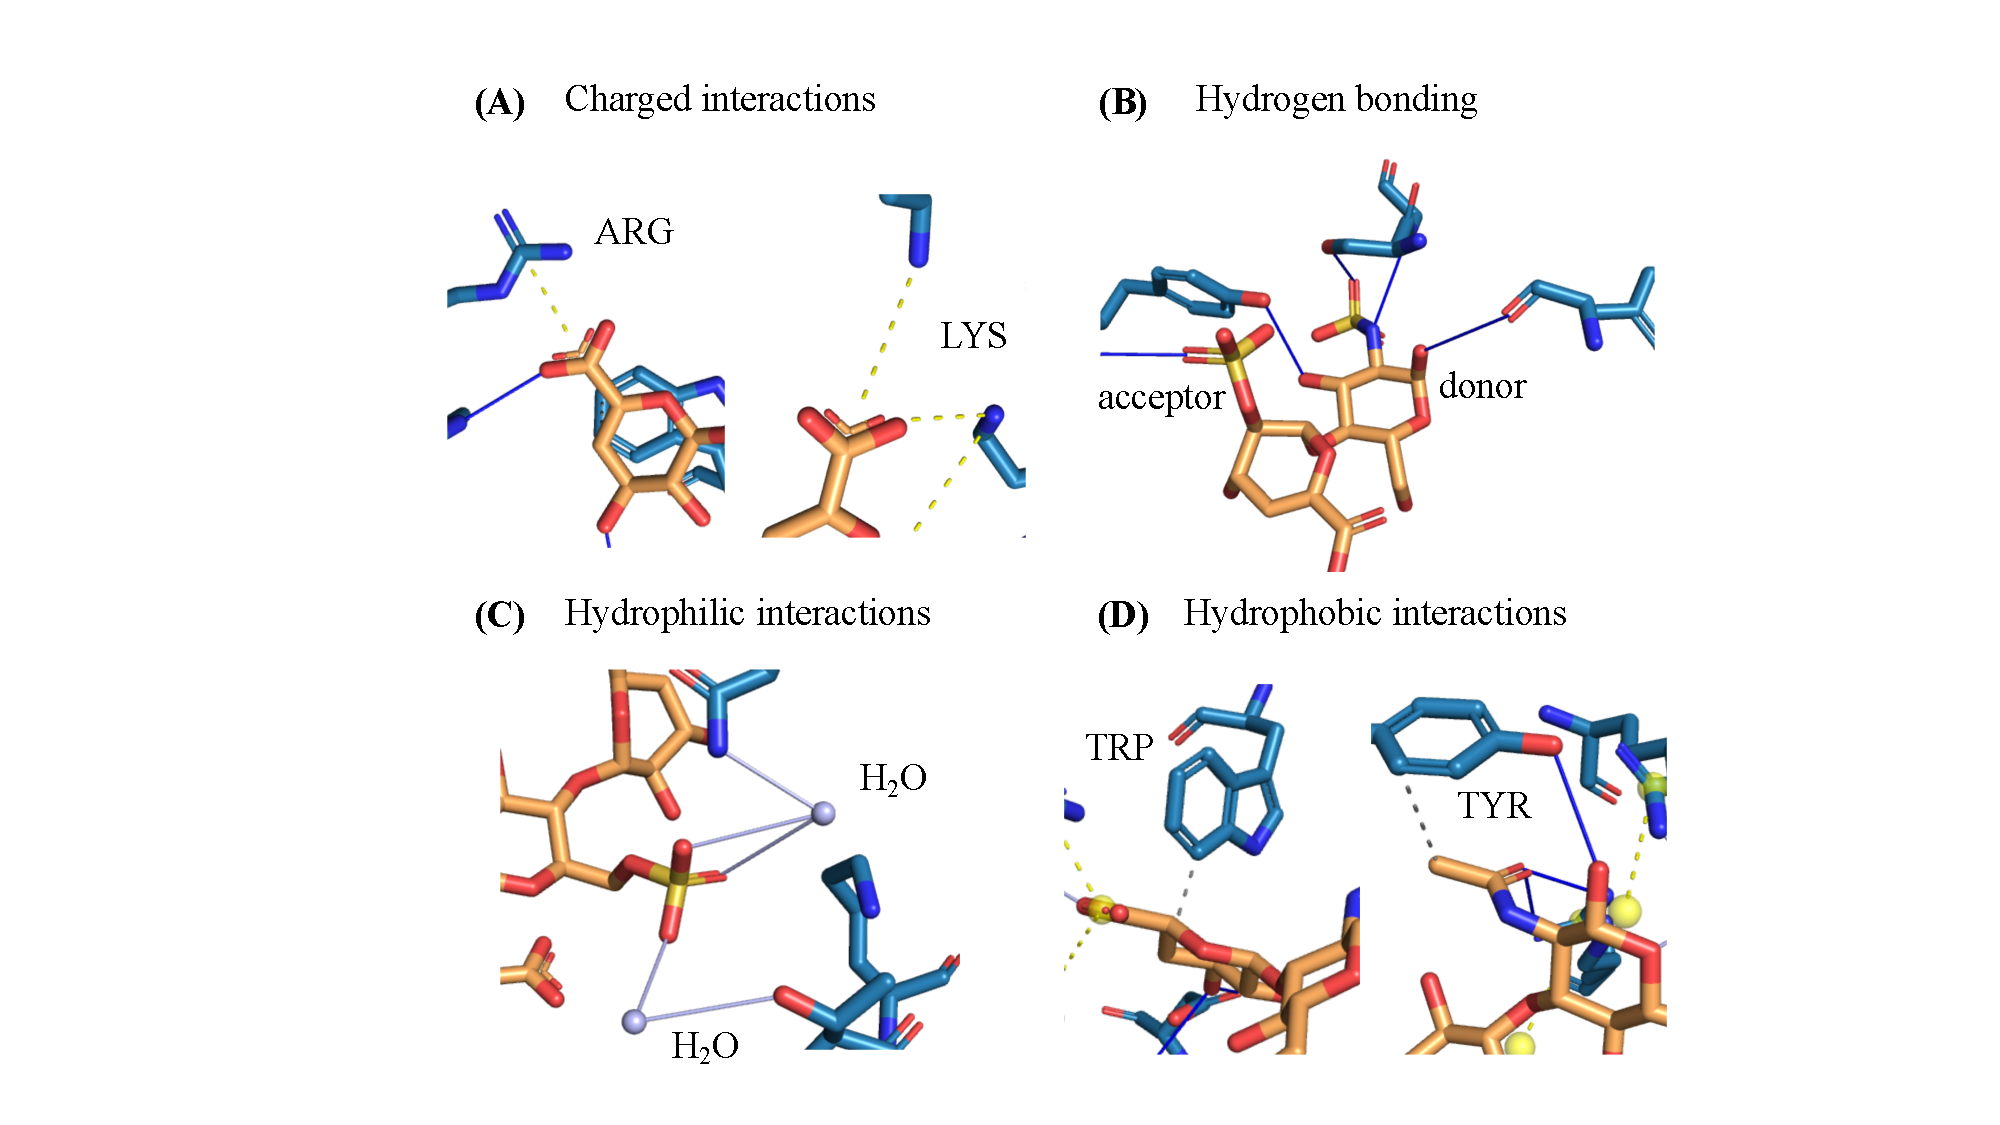
\includegraphics[width=11cm]{interactions.pdf}
    \caption{Examples of four types of non-covalent interactions between GAG--protein complexes, taken from the PDB. \textbf{(A)} Charged interactions, an important non specific interaction, are usually found between carboxylate/sulfonate groups and ARG, LYS or HIS (rare). \textbf{(B)} Hydrogen bonds are a common interaction, due to the large number of hydrogen bond donors/acceptors found in GAGs. \textbf{(C)} Due to their charge, GAGs are often solvated by water residues. \textbf{(D)} Hydrophobic residues, usually TRP or TYP, usually interact with GAGs \textit{via} C--H - - - \textpi~interactions.}
    \label{fig:interactions}
\end{figure}
\\
\\
\subsubsection*{~~~~~~~~~Hydrogen bonding}

Hydrogen bonding is the prevailing interaction to determine the specificity of \ac{GAG}--protein interactions.\cite{Taroni2000AnalysisSites} 
In general, carbohydrates form hydrogen bonds with side chain residues of polar planar amino acid residues to facilitate low energy conformations of the sugar.\cite{Malik2007SequenceNetwork, Quiocho1989Protein-carbohydrateFeatures}  
The free energy for hydrogen bonding can vary between −0.5 kcal mol$^{-1}$ (for neutral hydrogen bonds) to −4.7 kcal mol$^{-1}$ (for charged hydrogen bonds) \cite{Davis1997HydrogenHypothesis}. However, the contribution of a hydrogen bond to binding can be very modest (or penalizing) if the new interaction formed does not outweigh the desolvation penalty upon ligand binding. \cite{H.Williams1998AspectsInteractions}

\subsubsection*{~~~~~~~~~Solvation effects}

The thermodynamic consequences associated with desolvation of these highly charged oligosaccharides is trade-off that has an immense effect on the binding affinity of the ligand.\cite{Gandhi2009FreeInteractions, Samsonov2014FlexibilitySystems}
The desolvation penalty is large and positive and scales with increasing size and charge of the sugar.\cite{Gandhi2009FreeInteractions, Samsonov2014FlexibilitySystems} 
Ligand poses with favourable orientations of charged and hydrogen bond acceptor moieties are required to off-set this penalty and bind strongly with the protein. \cite{Bryce2001Carbohydrate-ProteinA}
For this reason, \ac{GAG} crystal structures are generally observed with a shell of water molecules partially covering portions of the ligand. \cite{Gandhi2009FreeInteractions, Capila2002Heparin-proteinInteractions.}

\subsubsection*{~~~~~~~~~Hydrophobic interactions}

Statistical analyses of general carbohydrate-binding protein sequences indicate that, for amino acids with hydrophobic side chains, Trp and Tyr are the the most highly represented. \cite{Malik2007SequenceNetwork, Sarkar2015AProteins, Shionyu-Mitsuyama2003AnProteins}. 
These residues have a significantly higher mean solvent accessibility in carbohydrate binding locations, whereas aliphatic residues (Ala, Gly, Ile and Leu) are more hydrophobic and not commonly found on the surface of proteins where sugar binding occurs. \cite{Malik2007SequenceNetwork, Shionyu-Mitsuyama2003AnProteins}. 
The aromatic rings of Tyr and Trp can pack against the hydrophobic face of a sugar molecule.\cite{Gandhi2008TheProteins} 
This can be seen in the \ac{PDB} (PDB entry 1I8Q and 1HM3, see figure \ref{fig:interactions} D). At certain orientations, \acp{GAG} can exhibit simultaneous hydrogen bonding and hydrophobic (C--H - - - \textpi) interactions with TYR.\cite{Li2001HyaluronanLyase., WeijunHuang2001ActiveMutagenesis}
Overall, the free energy of interaction, related to the observed dissociation constant (K$_{d}$), has contributions from the polyelectrolyte effect, hydrogen bonding, and hydrophobic interactions. \cite{Thompson1994EnergeticDomain}

% Structural similaries in 21 heparin-binding proteins, observed by Cardin and Weintraub, propose a consensus sequence of XBBXBX or XBBBXXBX, where B is a lysine or arginine (with a very rare occurrence of His) and X is a hydropathic residue, for heparin-binding proteins. When these Cardin--Weintraub sequences form \textalpha-helices, it is not uncommon for the spacing of these basic residues to allow for interactions on one face of the helix. \cite{Capila2002Heparin-proteinInteractions.} 
% Cardin and Weintraub sequences offer limited predictive value for heparin binding sites, as \acp{GAG}, in general, do not interact solely with one chain of the protein.\cite{Capila2002Heparin-proteinInteractions., Gandhi2008TheProteins} 
% Due to this, a 3D analysis of the binding site similarities is required. \cite{Sarkar2015AProteins}

\subsubsection{Deciphering the so-called `sulfation code'}

\begin{figure}[bl!]
    \centering
    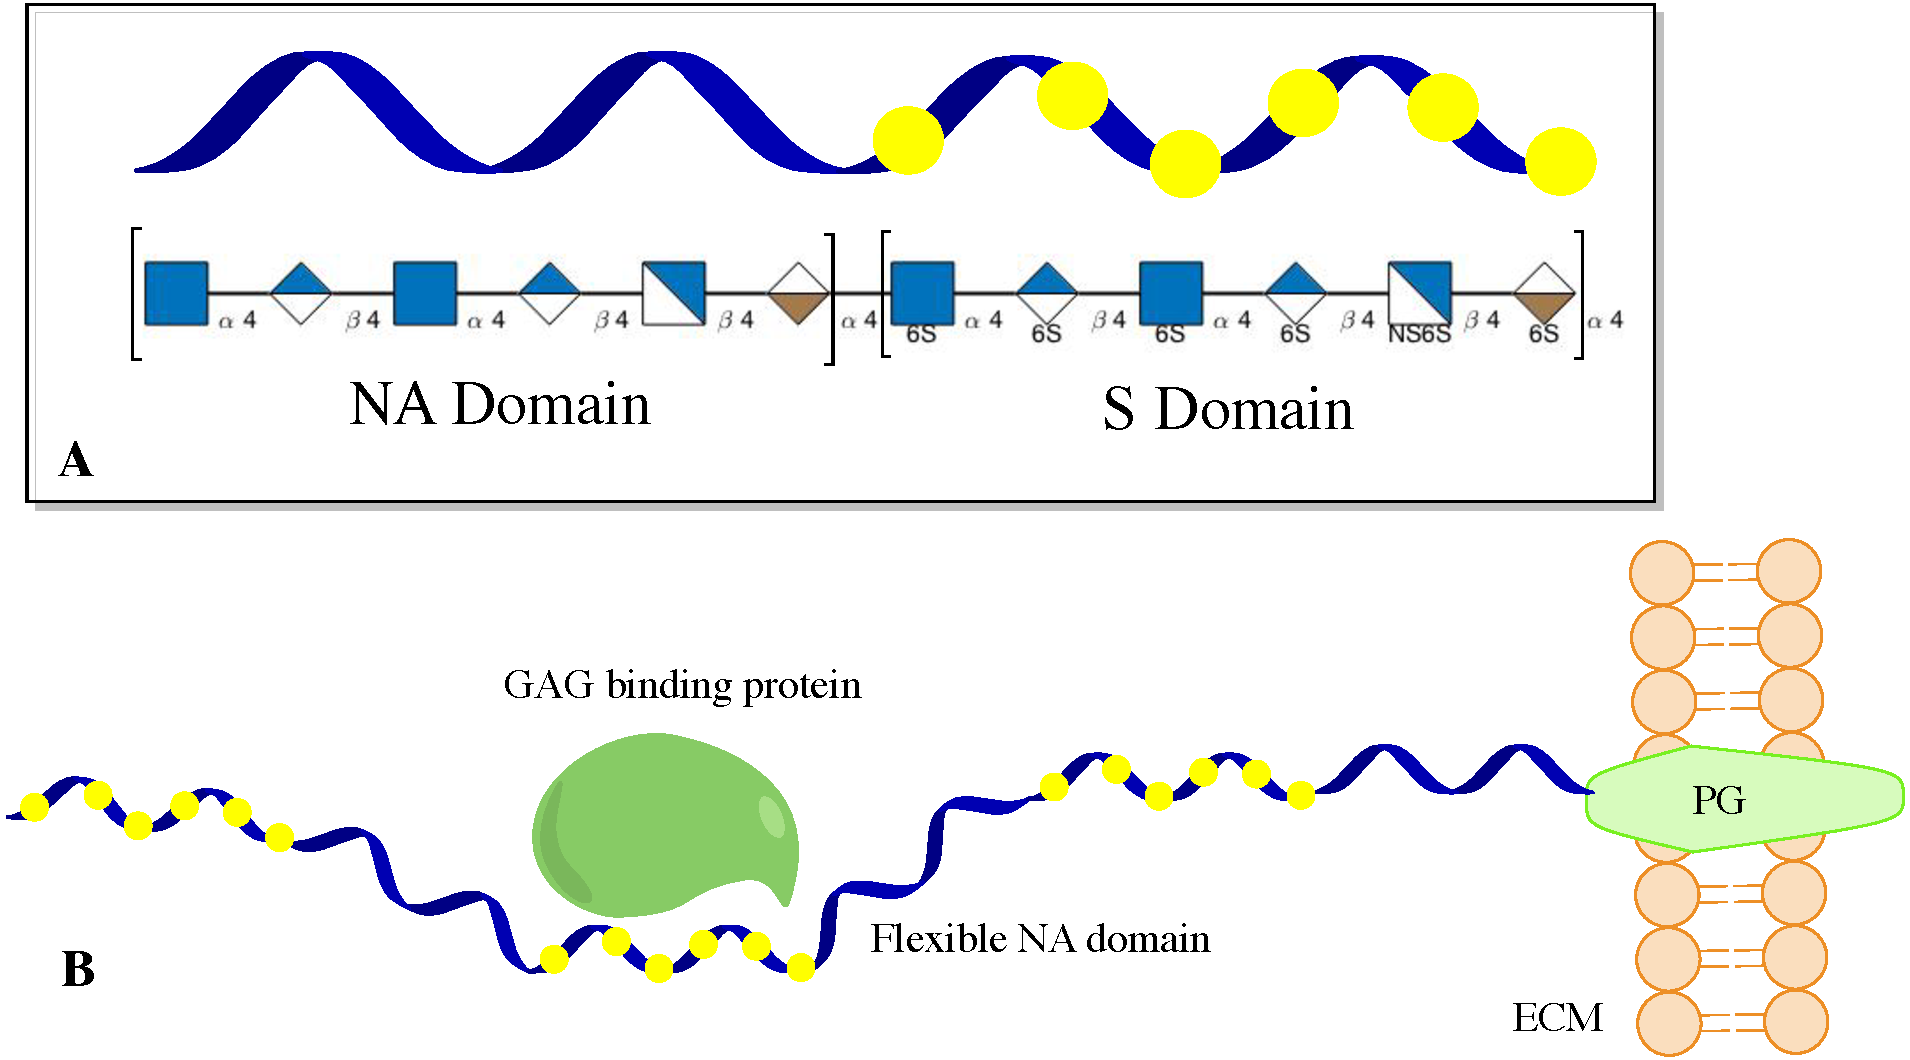
\includegraphics[width=13cm]{NAandSdomain.pdf}
    \caption{\textbf{(A)} Example of the GAG sequences (depicted in SNFG notation) showing the non-sulfated region (NA domain) and the sulfated region (S domain). \textbf{(B)} A cartoon representation of the induced fit between GAGs and proteins, faciliated by the flexable, non-sulfated domain.}
    \label{fig:Sdomain}
\end{figure}

Multiple \ac{SAR} studies related to \ac{GAG} sulfation patterns have suggested high specificity in relation to function.\cite{Habuchi2004SulfationCode, Gama2006SulfationActivity} 
In contrast, some \ac{GAG}--protein interactions have been shown to be entirely general (i.e. MIP-1\textalpha, an inflammatory protein, can be inhibited by sulfated oligosaccharides regardless of \ac{GAG} family. \cite{Kuschert1999GlycosaminoglycansResponses}
For this reason, GAG sulfation patterns have been likened to the “sulfation code”. \cite{Habuchi2004SulfationCode, Swarup2013SugarNeurons, Kowitsch2018MedicalReview, Gama2006SulfationActivity}
It is not only the specific sequences of sugars that effects GAG--protein interactions, but the sugars location in chain which also plays a role in this complex phenomenon. \cite{Capila2002Heparin-proteinInteractions.}
`Neighbourhoods' of varying sulfation levels in the oligosaccharide determine S and NA domains (sequences with high and low levels of sulfation respectively) (Figure \ref{fig:Sdomain} (A)). \cite{Gandhi2008TheProteins}
The conformation of IdoA is regulated by the sulfation pattern of itself and nearby saccharides. \cite{Hsieh2016Uncoveringe}
The 2-O sulfate groups of iduronic acid and 6-O and N sulfate groups on neighbouring hexosamine residues can strongly favour the $^{1}C_{4}$ Ido conformation, which causes a kink to the chain. \cite{Raman2005StructuralInteractions}
The NA domain has also been shown to introduce more flexibility to the chain and can allow the polymer to bridge across multiple binding sites of a protein (Figure \ref{fig:Sdomain} (B)). \cite{Capila2002Heparin-proteinInteractions., Nahain2018HeparinActivity, Li2004StructureHeparin, Dementiev2004TheSpecificity}

\begin{figure}[tl!]
    \centering
    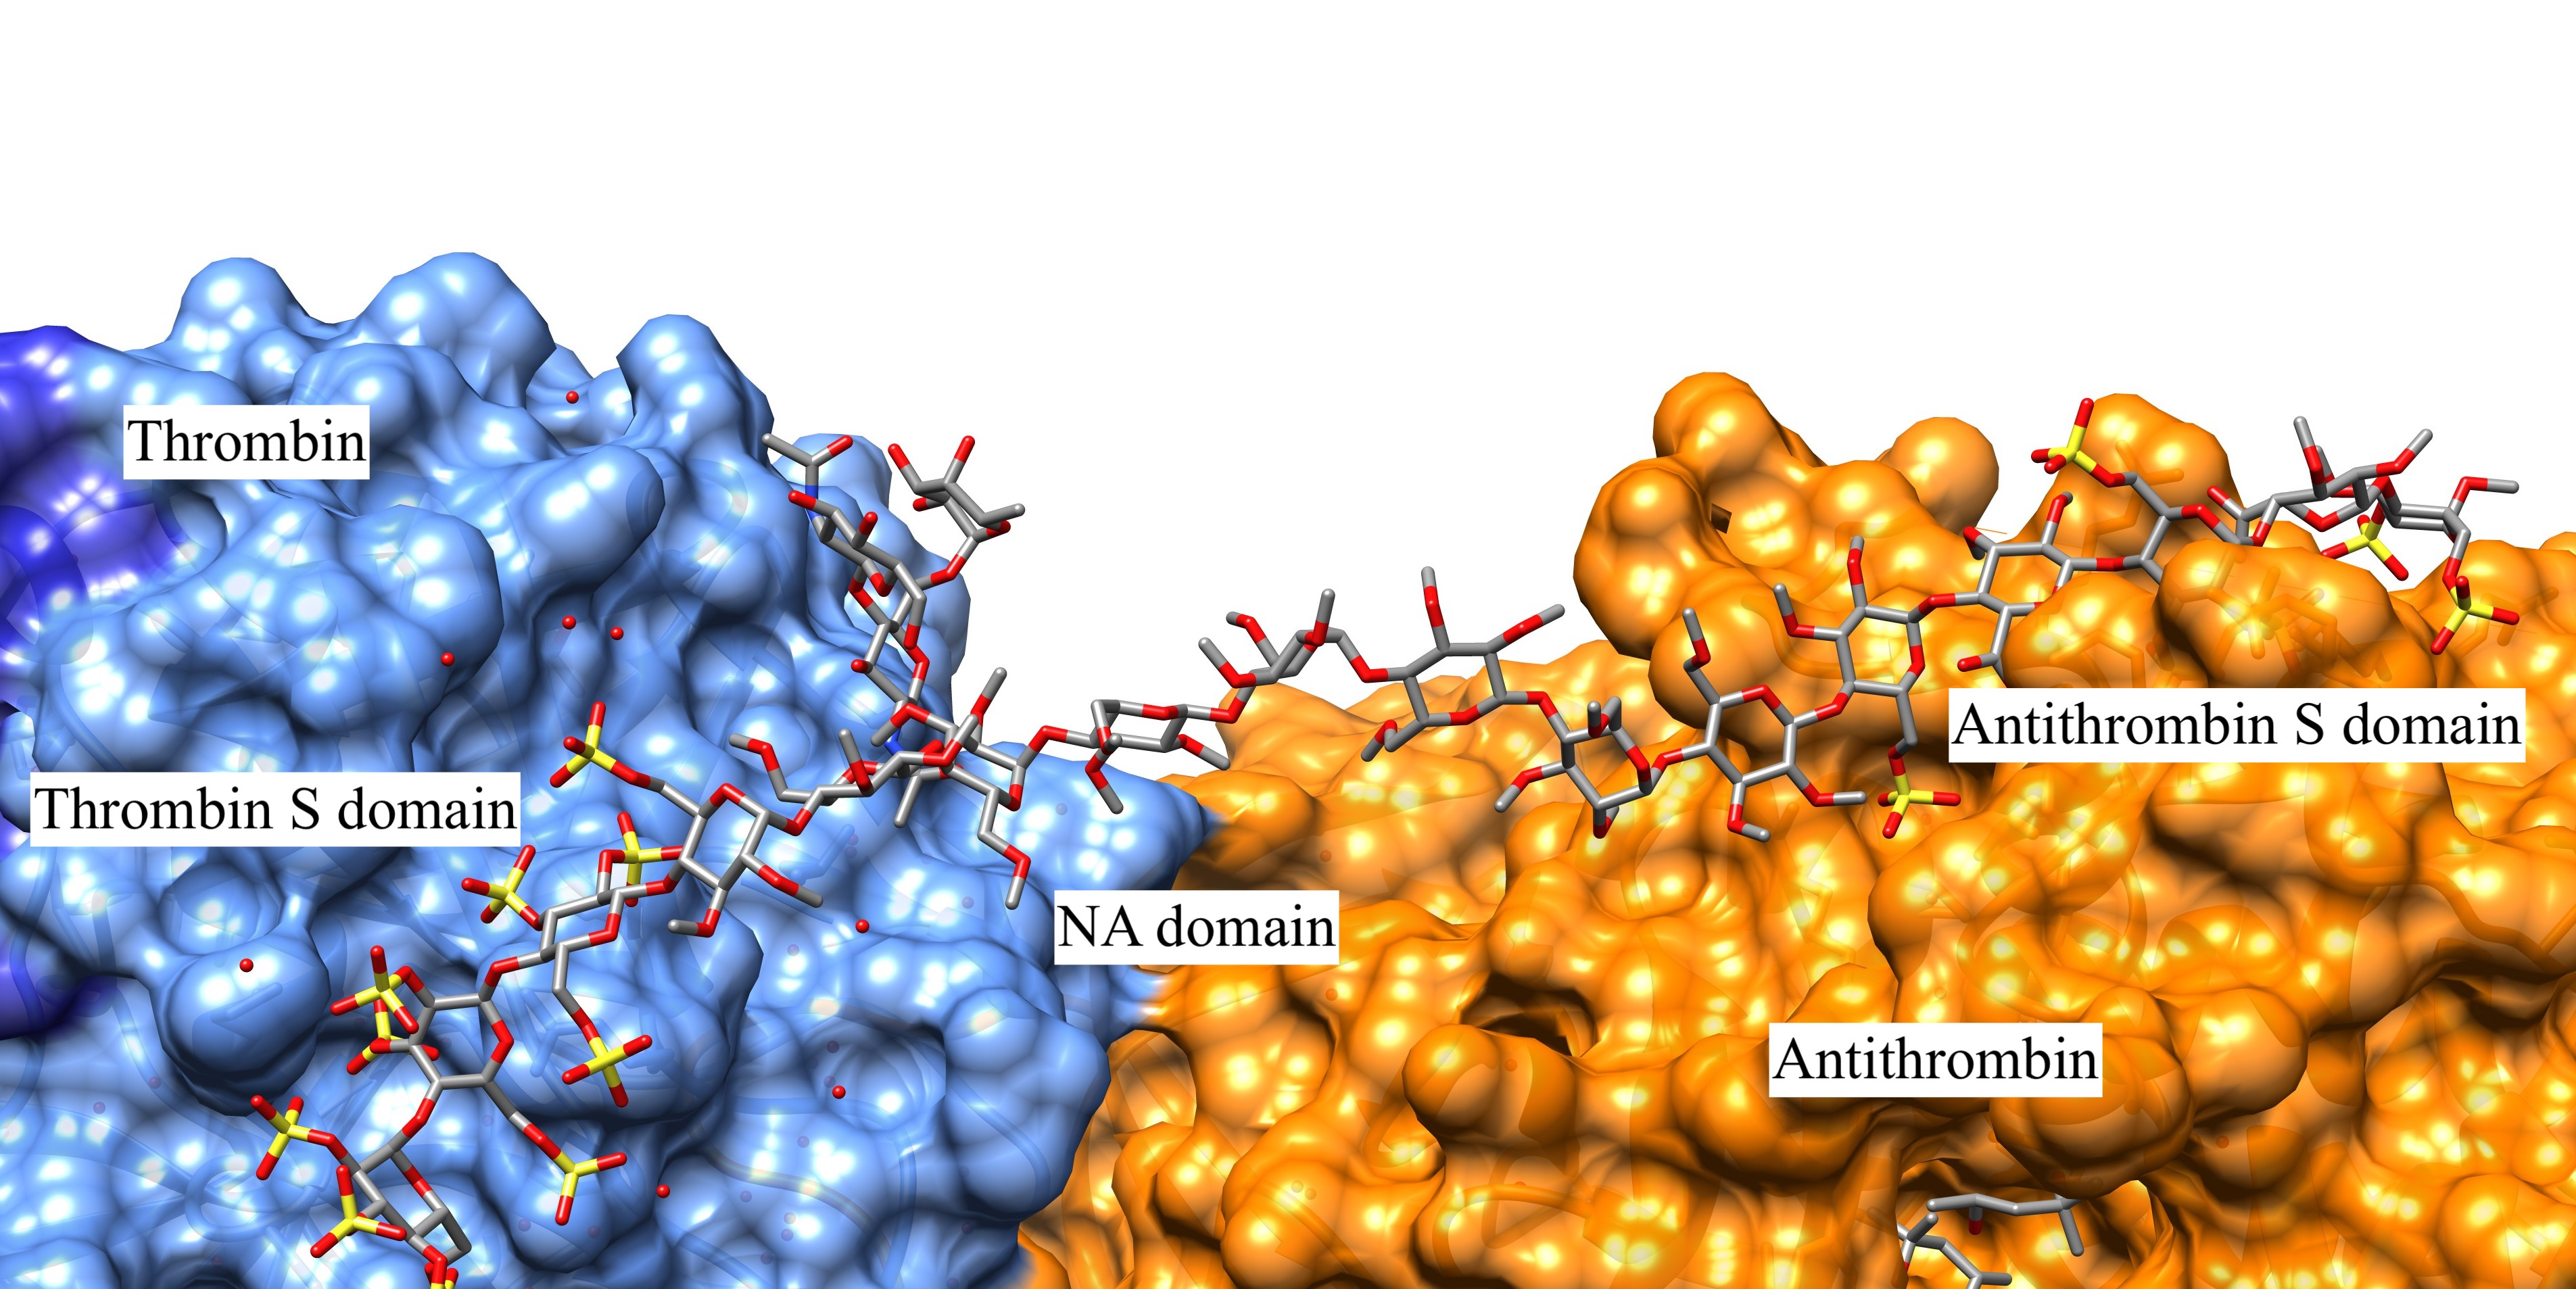
\includegraphics[width=13cm]{AntiThrombinThrombinHeparinMimetic.jpg}
    \caption{The ternary complex of antithrombin, thrombin and a 16-mer synthetic heparin mimetic, coloured by chain, showcasing the complimentary roles of S and NA domains during GAG binding, which can allow for recognition and flexibility, respectively (PDB entry 1TB6).}
    \label{fig:ternary}
\end{figure}

The prototypical example of this is the mechanism of thrombin inhibition which drives the efficacy of heparin as an anticoagulant. \cite{Li2004StructureHeparin, Dementiev2004TheSpecificity}
Antithrombin, the principal physiological inhibitor of thrombin, requires the formation of a ternary complex (antithrombin--heparin--thrombin) for inhibition to occur.\cite{Capila2002Heparin-proteinInteractions., Nahain2018HeparinActivity} In this complex, antithrombin recognizes a highly specific heparin pentasaccharide sequence through initial weak electrostatic interactions which causes a conformational change. \cite{Li2004StructureHeparin}
If the heparin polymer is sufficiently long and flexible it can bind non-specifically to thrombin on the opposite side of the chain.\cite{Dementiev2004TheSpecificity}
The thrombin protein can direct itself towards antithrombin in the correct orientation, effectively using the oligosaccharide chain as a guide rope.\cite{Li2004StructureHeparin, Dementiev2004TheSpecificity} This assistance provided by oligosaccharide increases the antithrombin induced inhibition of thrombin by 4000 fold. \cite{Li2004StructureHeparin, Dementiev2004TheSpecificity} 
This ternary complex has been characterized with synthetic 16-mer heparin mimetic using x-ray crystallography (Figure \ref{fig:ternary}, PDB entry 1TB6).\cite{Dementiev2004TheSpecificity}

Due to the immense variation of \acp{GAG}, isolating defined sulfation sequences from biological sources is difficult and often a task for the synthetic chemist.  \cite{Gama2006SulfationActivity}
These synthetic procedures are generally non-trivial. \cite{Das2001SynthesisHeparin} 
The methods available for characterization of 
\ac{GAG}--protein interactions at the atomistic level (x-ray crystallography and protein NMR) are not suitable for high-throughput analysis of \acp{GAG}. \cite{Sankaranarayanan2018SoAgain}
This pushes the problem of rationalizing \ac{GAG}--protein interactions into the hands of computational chemists and necessitates the development of computational techniques for understanding these essential biomolecules. \cite{Woods2018PredictingComplexes, Sankaranarayanan2018SoAgain}


% Carbohydrates in computation
% Carbohydrates in computation
% Carbohydrates in computation
% Carbohydrates in computation
% Carbohydrates in computation
% Carbohydrates in computation
% Carbohydrates in computation
% Carbohydrates in computation
\pagebreak
\subsection{Carbohydrates in computational chemistry}
\subsubsection{Overview}

\begin{figure}[bl!]
    \centering
    \includegraphics{"computational techniques".pdf}
    \caption{An explanation and comparison of three computational techniques: quantum mechanics, molecular dynamics and docking. The limitations of each method, and how each method can be used in conjunction to mitigate said limitations, is highlighted.}
    \label{fig:comp}
\end{figure}


Computational chemistry techniques which attempt to calculate the free energy of a system can be separated into two classes: \ac{QM}, where the electron is the smallest particle of interest; and \acf{MD}, where the smallest particle is the atom. \cite{Jensen2007IntroductionEdition, Dror2012BiomolecularBiology}
For problems such as probing chemically interesting \ac{GAG}--protein interactions, nonempircal methods, such as `docking', can be used -- trading off the accuracy of \ac{QM}/\ac{MD} free energy calculations for speed by using scoring functions to rank suspected low energy poses. \cite{Halperin2002PrinciplesFunctions}
These methods are summarized in Figure \ref{fig:comp}.

To quantify the efficiency of these computational techniques, it is convenient to introduce a notion from computer science: time complexity (commonly represented as $\mathcal{O}(f(n))$).\cite{Goldreich2008ComputationalComplexity} Time complexity relates the size of a task, $n$, to the time taken to complete the task, $f(n)$ (see Figure \ref{fig:timecomplexity}).\cite{ButterfieldAScience} The units of size and time are arbitrary and should be defined by the author. Highly accurate \ac{QM} calculations scale $\mathcal{O}(n^{7})$ (where n is the number of model electronic orbitals), while simple energy scoring functions in docking programs can be as efficient as $\mathcal{O}(n^{2})$ (n being the number of heavy atoms). \cite{Jensen2007IntroductionEdition, Engler2018Multiple-ChoiceMolecules, Krippahl2005ApplyingDocking} 
The time complexity of \ac{MD} simulations, based on system size, falls in between \ac{QM} and docking, depending on the types of forces modelled. Determination of hydrogen bonding and electrostatic free energies can be efficient as $\mathcal{O}(n^{2})$ and $\mathcal{O}(n \log n)$, respectively.\cite{Trobec1997TheAlgorithms} The ultimate benefit of MD simulations is that the processing time usually scales linearly, $\mathcal{O}(n)$, with the timestep of the simulation.\cite{Anderson2008GeneralUnits}

\begin{figure}[tl!]
    \centering
    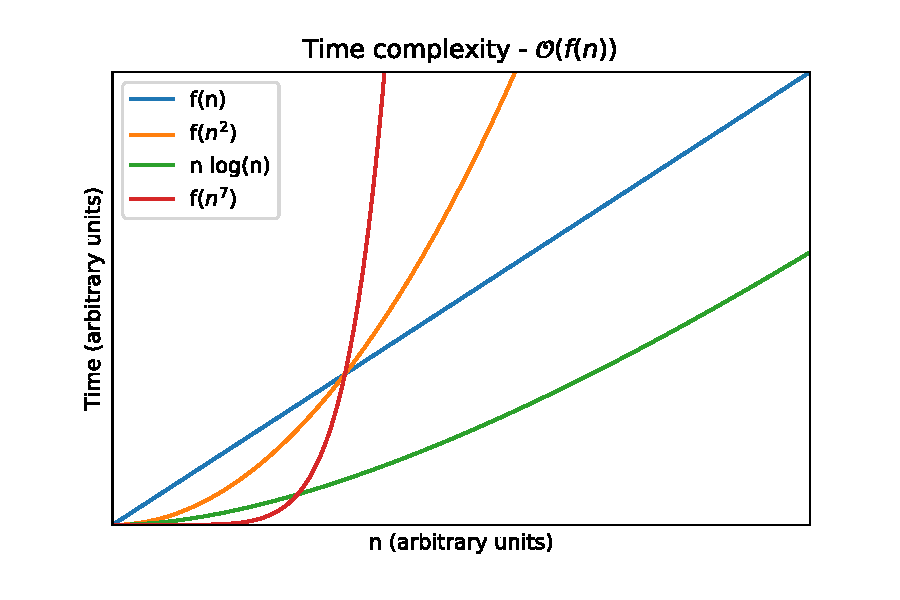
\includegraphics[width=9cm]{timecomplexity.pdf}
    \caption{Visualization of selected time complexity relationships, i.e. $\mathcal{O}(f(n))$, relevant to computational chemistry. }
    \label{fig:timecomplexity}
\end{figure}

The internal, rotational degrees of freedom of a molecule can have a profound impact on the time complexity of computational techniques.\cite{Halperin2002PrinciplesFunctions}
Molecular conformational space can be considerably large and scales exponentially with system size.\cite{Zsoldos2007EHiTS:System}
For an average sized ligand with 6 rotatable bonds in a 10 \AA$^{2}$ box there are expected to be approximately 10$^{20}$ possible poses (when sampling angles in increments of 5\textdegree~and translations in increments of 0.5 \AA).\cite{Zsoldos2007EHiTS:System}
Since oligosaccharides possess more than 6 rotatable bonds on average, conformational space of sugars is generally larger. \cite{Nivedha2016Vina-Carb:Docking}
The size of conformational space can prohibit brute force sampling of every possible rotamer to find a low energy solution. \cite{Zsoldos2007EHiTS:System}
\ac{QM} and \ac{MD} find low energy conformations using empirical energy calculations to perform structure refinement when given enough iterations.\cite{Jensen2007IntroductionEdition, Dror2012BiomolecularBiology}
However, their computational cost makes them nonviable for the high-throughput search of computational space when exploring protein--ligand interactions. \cite{Jensen2007IntroductionEdition, Engler2018Multiple-ChoiceMolecules}
Docking programs, which rely on `search algorithms' to restrict the conformational search space, are optimized for speed and are generally the first port of call for this task. \cite{Halperin2002PrinciplesFunctions, Bostrom2001ReproducingTools} 

% The uses and limitations of each method, and how each method can be used in conjunction to mitigate these limitations, should be understood (see Figure \ref{fig:comp}).


\subsubsection{Protein--ligand docking}

\epigraph{Given the atomic coordinates of two molecules, predict their “correct” bound association.}{The `molecular docking problem' as defined by Halperin \textit{et al}.\cite{Halperin2002PrinciplesFunctions}}

{\setlength\parindent{0pt} Docking can be compartmentalized into two main procedures: the search algorithm, which aims to find low energy poses; and the scoring function, which aims to rank these poses.\cite{Halperin2002PrinciplesFunctions, Schulz-Gasch2004ScoringPerspective, Pagadala2017SoftwareReview} 
Scoring can be performed after each pose is generated or after the search algorithm is complete. \cite{Halperin2002PrinciplesFunctions} 

}
% Validation of these poses is usually performed by \ac{RMSD} comparison between known crystal structures.\cite{Nivedha2016Vina-Carb:Docking}} 

\subsubsection*{~~~~~~~~~Search algorithms}

The choice of search algorithm usually depends on whether the binding site of the ligand is known. If not, the approach is generalized as `blind docking' and prediction of the binding site is performed using a method known as site-mapping. Protein homology can be an effective technique for predicting binding sites when analogous binding sites have been characterized.\cite{Gandhi2012PredictionBMPs, Agostino2014DevelopmentGlycosaminoglycans, Mottarella2014DockingProteins, Hileman1998Glycosaminoglycan-proteinProteins}
\footnote{Experimental data to infer binding sites include NMR experiments\cite{Pomin2018Glycosaminoglycan-ProteinSpectroscopy} (such as saturation transfer difference (STD)\cite{Haselhorst2007STDCore} or transferred nuclear Overhauser enhancement (tr-NOE)\cite{Mobius2013InvestigationApproach}), protein mutagenesis studies\cite{WeijunHuang2001ActiveMutagenesis} and crystallography.\cite{Huang1999CrystalResolution}}
Entire docking programs are dedicated to site-mapping\cite{Mottarella2014DockingProteins, Peters1996TheCriteria, Comeau2007ClusPro:Server} yet the accuracy of these methods are commonly disputed.\cite{Sankaranarayanan2018SoAgain} 
If the answer the question is yes, the search space of the putative binding site can be reduced, allowing for more rigorous and computationally expensive search algorithms.\cite{Halperin2002PrinciplesFunctions} 
Common search algorithms are \ac{MC} (or random sampling), \ac{MD} search (which simulate a trajectory of the ligand in the binding pocket) and \ac{GS} (which mimics the biological process of evolution by iterative selection of pose features that improve the binding efficiency of the complex). 
Out of these approaches, \Ac{GS} algorithms are the most computationally expensive; however, out of the algorithms listed they can be the most effective at sampling the entire computational space.\cite{Morris1639AutomatedFunction, Halperin2002PrinciplesFunctions}
Two examples of \ac{GAG} specific approaches to search algorithms employed in the literature have been identified:

1. The Cluspro server is an online protein--protein docking package which was adapted in 2014 to include a tool for \ac{Hep} site mapping.\cite{Comeau2007ClusPro:Server, Mottarella2014DockingProteins,Kozakov2017TheDocking.} 
Cluspro performs three main computational procedures: \ac{RBD}, \ac{RMSD} clustering and refinement using an energy minimization function.\cite{Kozakov2017TheDocking.} In the \ac{RBD} step, the protein and ligand (a generic heparin tetramer: Ido2S-(\textalpha1-4)-GlcNS6S-(\textbeta1-4)-Ido2S-(\textalpha1-4)-GlcNS6S) are treated as inflexible. Since the ligand has no internal degrees of freedom, the entire surface area of the protein can be sampled by moving the ligand around the protein on a 3D grid with 1\AA~spacing. \cite{Mottarella2014DockingProteins} 
At each grid point, the ligand is rotated 70000 times. \cite{Mottarella2014DockingProteins} 
This step is followed by clustering ligands using \ac{RMSD} and evaluating representative structures from these clusters using a combined energy and shape complimentarity scoring function adapted from the ZDOCK program.\cite{Kozakov2017TheDocking., Chen2003ZDOCK:Algorithm}
Since the server only allows site mapping of one specific heparin tetramer, its general utility for \ac{HS} or \ac{Hep} analogs is questionable. 
Further analysis using more rigorous docking or \ac{MD} at these sites is required to better understand atomistic protein--ligand interactions. \cite{Mottarella2014DockingProteins} 

2. The ``GAG-Dock" method reported by Griffith \textit{et al.}\cite{Griffith2017PredictingGrowth} was developed using DarwinDock and GenDock to model \ac{GAG}--protein interactions. It presents a method of reducing the search space by sampling exclusively from flat regions of the protein (where \ac{GAG} binding sites are typically localized), using a \ac{GS} approach.\cite{Griffith2017PredictingGrowth}
These flat surfaces were identified using topological analysis with a modified version of the program `Sphgen'.\cite{Moustakas2006Development5, Hendrix1998SurfaceDocking.}
After clustering and energy scoring using the DRIEDING forcefield\cite{Mayo1990DREIDING:Simulations}, this method accurately predicted \ac{Hep} binding poses between 0.60 - 1.51 \r{A} \ac{RMSD} of the three crystal structures (fibroblast growth factors 1 and 2, and \textalpha-antithrombin III).\cite{Griffith2017PredictingGrowth} 
While these predictions are highly accurate, the small sample size (3) of flat binding sites likely lent themselves to efficient sampling using their specialized technique and it remains to be seen if these results can be generalized for all \ac{GAG} complexes.\cite{Griffith2017PredictingGrowth}

\subsubsection*{~~~~~~~~~Scoring functions}

The ideal docking scoring functions should rank poses based on binding free energies, however no contemporary scoring function comes close to accomplishing this task.\cite{Schulz-Gasch2004ScoringPerspective}
The gold standard of scoring functions presented in the literature are force field based energy scoring functions. Similar to \ac{MD} force fields (discussed in Section \ref{MD}), approximate binding free energies are modelled as the sum of independent energy terms (i.e. electrostatic and van der Waals interactions), some of which can be determined by \ac{QM} calculations (discussed in Section \ref{QM}).\cite{Schulz-Gasch2004ScoringPerspective}
The pitfalls of this approach include the overestimation of repulsive and polar interactions, and failure to account for the impact of solvation free energies. \cite{Gandhi2009FreeInteractions, Schulz-Gasch2004ScoringPerspective, Dommert2012ForceDevelopments, Shoichet1999LigandDocking}
Other commonly implemented scoring functions include empirical scoring functions, which correlate protein--ligand crystal structures to known $K_{i}$ (inhibitory concentration) values to approximate energetics (usually of hydrogen bonding and hydrophobic interaction terms); and knowledge based scoring functions, which use statistical analysis of crystal structures to create a method to classify likely binding distances between atoms.\cite{Schulz-Gasch2004ScoringPerspective}
Two examples of carbohydrate specific scoring functions have been identified in the literature:

1. The SLICK (Sugar--Lectin Interactions and doCKing) scoring method, which was implemented into the BALLDOCK docking software, developed a empirical scoring function calibrated using a set of ten carbohydrate--lectin complexes with experimental binding energies.\cite{AndreasKerzmann2006SLICKInteractions, Kerzmann2008BALLDock/SLICK:Docking}
The terms in the scoring function include contributions from CH - - -\textpi~interactions, hydrogen bonding, van der Waals and electrostatics.\cite{Neumann2004ComputationalInteraction, AndreasKerzmann2006SLICKInteractions} The score S is given by:
\begin{equation} \label{eq:1}
S = s_0 + s_{CH\pi}\cdot S_{CH\pi} + s_{hb}\cdot S_{hb} + s_{vdW}\cdot \Delta E_{vdW} + s_{es}\cdot \Delta E_{es}^{Coulomb}
\end{equation}
Where $s_{0}$ represents a correction factor and the following $s$ values represent the weight of the specified interaction and each $S$ represents the specific scoring function for each interaction.\cite{AndreasKerzmann2006SLICKInteractions} The specific scoring functions were created using linear regression to correlate geometric properties relevant to the interaction with the binding coefficient.\cite{AndreasKerzmann2006SLICKInteractions, Kerzmann2008BALLDock/SLICK:Docking}
The weights were calibrated manually to fit the data.\cite{AndreasKerzmann2006SLICKInteractions}
Docking a GlcNAc trimer and tetramer (PDB entry 1EHH and 1EN2) resulted in top ranked structures with fairly low RMSD ($<$ 1.5 \AA).\cite{AndreasKerzmann2006SLICKInteractions, Kerzmann2008BALLDock/SLICK:Docking} 
These complexes were reportedly strongly influenced by CH - - - \textpi~interaction interactions, which the researchers attributed to the successful poses.\cite{AndreasKerzmann2006SLICKInteractions, Kerzmann2008BALLDock/SLICK:Docking}
However, due to the small sample size (10) of the calibration data set, there is undeniable over-fitting of the model.\cite{AndreasKerzmann2006SLICKInteractions, Kerzmann2008BALLDock/SLICK:Docking}
Therefore, it is highly unlikely that this model will translate well to \acp{GAG}.\cite{Samsonov2016ComputationalComplexes}

2. The \ac{CHI} energy penalty function (the only carbohydrate specific energy function to date) and has been integrated into the preexisting C++ source code of \ac{ADV}.\cite{Nivedha2015CarbohydrateChaff, Nivedha2016Vina-Carb:Docking} This modified code has been titled VinaCarb. Although \ac{ADV} uses a considerably expensive \ac{GS} algorithm, it has been highly optimized to run on multiple CPUs and dramatically outperforms its predecessor, \ac{AD4}, in speed and accuracy.\cite{Trott2010SoftwareMultithreading} A recent comparison of docking programs, which included \ac{AD4}, \ac{ADV}, MOE, eHITS, FlexX and Glide, found \ac{ADV} produced the lowest structural differences between all analyzed poses and the crystal structure for a dataset containing \ac{Hep} and \ac{HS} and was also the program that best correlated docking score to \ac{RMSD}.\cite{Samsonov2016ComputationalComplexes} Since VinaCarb shares the base \ac{ADV} scoring function, these data suggests that VinaCarb may be effective at docking \acp{GAG}.  

The \ac{CHI} energy penalty function aims to discriminate poses based on carbohydrate \textphi~and \textpsi~ torsions (discussed in Section \ref{structure}). Since these torsions are expected to fall inside a small range,\cite{Woods2018PredictingComplexes, Nivedha2015CarbohydrateChaff} systematically excluding poses with torsions outside this range would drastically decrease the size of the comformational search space required. Rotational energy profiles for carbohydrate \textphi~and \textpsi~ torsions were calculated using \ac{QM}, specifically at the B3LYP/6-3111G(2d,2p) level of theory, performed after geometry optimization at the HF/6-31G(d,p) level of theory, in increments of 15\textdegree~(the suitability of these methods is discussed in section \ref{QM}).\cite{Nivedha2015CarbohydrateChaff, Nivedha2016Vina-Carb:Docking} 
Since the number of heavy atoms in a simple disaccharide (e.g. maltose = 33) requires a significant computational cost, \ac{THP} was used instead to model a carbohydrate ring. 1-2, 1-3 and 1-4 glycosidic linkages for all \textalpha~and \textbeta~anomers, and axial and equitorial linkage isomers) were modeled using two \ac{THP} molecules.\cite{Nivedha2015CarbohydrateChaff, Nivedha2016Vina-Carb:Docking} 
These calculations were done using the $^{4}C_{1}$ and $^{1}C_{4}$ configurations of \ac{THP}. The frequency of glycosidic torsion angles in the \ac{PDB} were found to correlate to the minima in the rotational energy profile. In general, carbohydrate--protein complexes are believed to crystalize in low energy conformations.\cite{Nivedha2015CarbohydrateChaff, Nivedha2016Vina-Carb:Docking}
These data suggest that the \ac{CHI} energy function may be a suitable model for predicting low energy binding conformations. VinaCarb identified poses with $<$ 2 \AA~\ac{RMSD} from the the crystal structure 74\% of the time, compared to 55\% when using \ac{ADV}.\cite{Nivedha2016Vina-Carb:Docking}
As demonstrated by VinaCarb, carbohydrate specific scoring functions can greatly improve the prediction of carbohydrate crystal structures.\cite{Nivedha2015CarbohydrateChaff, Nivedha2016Vina-Carb:Docking} However, its energy function fails to take into account $^{2}S_{O}$ ring conformations, which are necessary to score oligosaccharides containing IdoA. 

\subsubsection*{~~~~~~~~~A critique of docking} \label{critique}


Scoring functions provide varying results due to their inherent simplifications. 
Docking has an inherent flaw that must be accounted for.
Realistically, only conformations with experiment (i.e. NMR or crystallography) or support using judicious \ac{MD} simulation, is the only way to truly score the likelihood of docking poses.\cite{Samsonov2016ComputationalComplexes, Nivedha2016Vina-Carb:Docking, Sankaranarayanan2014TowardProteins}


\subsubsection{Molecular dynamics} \label{MD}

Calculating the free energy of biological systems using \ac{QM} methods is computationally unfeasible.\cite{Dror2012BiomolecularBiology}
\ac{MD} simplifies energy calculations by creating energy functions, or force fields, that 
compute the interatomic forces as pairwise additive functions that contribute to the total free energy.\cite{Dror2012BiomolecularBiology, Woods2010ComputationalComplexes} 
Most force fields are similar in form to equation \ref{eq:2}\footnote{a, b, c and d refer to individual atoms.}:
\begin{equation} \label{eq:2}
\begin{multlined}
V(r_{1}, ..., r_{N}) = \sum_{a<b}V_{Bonds}(r_{a, b})~+~ 
\sum_{a<b<c}V_{Angles}(\theta_{a, b, c})~+ 
\sum_{a<b<c<d}V_{Torsions}(\varphi_{a, b, c, d})~+~
\\
\sum_{a<b}V_{Coulomb}(r_{a, b})~+~\sum_{a<b}V_{vdW}(r_{a, b})
\end{multlined}
\end{equation}
where: 
\begin{equation} \label{eq:3}
V_{Bonds}(r_{a, b}) =  \frac{1}{2} \cdot k^{b}_{ab}(k_{ab}-k^{0}_{ab})^{2}
\end{equation}
\begin{equation} \label{eq:4}
V_{Angles}(\theta_{a, b, c}) = 
\frac{1}{2}  \cdot k^{\theta}_{ab}(\theta_{abc}-\theta^{0}_{abc})^{2}
\end{equation}
\begin{equation} \label{eq:5}
V_{Torsions}(\varphi_{a, b, c, d}) = \frac{1}{2}  \cdot k_{\varphi} (1+\cos(n\varphi+\gamma))
\end{equation}
\begin{equation} \label{eq:6}
V_{Coulomb}(r_{a, b}) = \frac{1}{4\pi \epsilon_{0}} \cdot \frac{q_{a}q_{b}}{\epsilon_{r} r_{ab}}
\end{equation}
\begin{equation} \label{eq:7}
V_{vdW}(r_{a, b}) = 4\epsilon \Bigg[ \bigg(\frac{\sigma_{ab}}{r_{ab}} \bigg) ^{12} - \bigg( \frac{\sigma_{ab}}{r_{ab}} \bigg) ^{6} \Bigg]
\end{equation}
However, simillar to parameterizing scoring functions, the techniques used to set the parameters (k, q, etc.) differ.\cite{Woods2010ComputationalComplexes}
These functions allow for the energy contributions of individual residues to be determined easily. The evolution of these forces over time is treated using classical mechanics, allowing for the estimation of kinetic and thermodynamic properties of biological system. Carbohydrate specific forcefields, and their associated \ac{MD} simulation packages, include GLYCAM (AMBER) and 53A6$_{GLYC}$ (GROMOS). These force fields have been successful at reproducing ring flipping and NMR observables. 

\ac{MD} simulations of \ac{GAG}--protein crystal structures found these structures to be stable (i.e. these ligands did not leave the binding pocket) over time (20 ns). However, specific hydrogen bonding and electrostatic interactions were not retained over the course of the simulation. Similarly, \ac{MD} can be employed to eliminate false positives generated from \ac{GAG} docking and can provide reasonable estimates of binding coefficients and free energies to score docking results. One crucial drawback is that \ac{MD} tends to overestimate free energies as the size of the ligand increases. To mitigate this effect, free energies can be standardized by the number of monomers in an oligosaccharide.

\subsubsection{Quantum mechanics} \label{QM}

The underlying goal of \ac{QM} in computational chemistry is to provide an approximate\footnote{The exact form of the Schrodinger wave equation is infinite and its time complexity scales exponentially. Therefore it is insoluble using brute force computational techniques.} solution to the Schrodinger wave equation when given the positions of nuclei and the number of their electrons.
\ac{QM} methods also require basis sets, which are functions that represent the type of electronic orbitals modelled in the calculation.
\textit{Ab initio} \ac{QM} methods that take into account electron correlation, such as CCSD(T) and MP2, can provide highly accurate estimates of thermodynamics and molecular geometries when compared to experimental results. Kohn--Sham \ac{DFT} is an extremely popular \ac{QM} methodology that approximates the Schrodinger wave equation by modelling electron density and can also provide accurate results at a fraction of the cost of \textit{ab initio} methods. However, not all DFT methods are suitable for modelling carbohydrates. B3LYP, which was used for the parameterization of the VinaCarb \ac{CHI} energy function, was one of the worst performing methods in recent benchmarking studies that compared a range of methods to CCSD(T) and MP2 for model carbohydrate systems (glucose and \textalpha-maltose).
The MO6-2X and PBE0, which are relatively similar in cost to B3LYP, have been shown better correlation with high level \textit{ab initio} methods.  
Similarly, while the basis set used in the parameterization of the \ac{CHI} energy function was relatively large, it neglected to include a diffuse function, which has been shown to aid models of anionic systems). Finally, while \ac{QM} calculations for the \ac{CHI} energy function were done in the gas phase, an implicit aqueous solvent would likely be more appropriate for modelling carbohydrate--protein interactions.

\pagebreak
\section{Aims}

The aims of this investigation are to: \textbf{(1)} perform statistical analysis of structural features of \ac{GAG}--protein structures in the PDB through the development of novel computational tools, \textbf{(2)} develop a \ac{GAG} specific scoring function that correlates glycosidic torsions to internal energies, \textbf{(3)} benchmark the VinaCarb \ac{CHI} energy function, and the novel \ac{GAG} scoring function, against experimental \ac{GAG}--protein crystal structures.

\section{Methods}

\ac{GAG} structure analysis tools will be developed using the Python programming language and be aimed at analyzing crystal structures and \ac{MD} simulation trajectories.
\textphi~and \textpsi~rotational energy profiles of $^{4}C_{1}$, $^{1}C_{4}$ and $^{2}S_{O}$ disaccharide models (using \ac{THP}) will be calculated with the MO6-2X and PBE0 functionals, using 6-311G++(2d,2p) (and larger) basis sets and an implicit solvent model (water). These calculations will be performed using the Gaussian16 quantum chemistry program. Correlation between crystal structures and low energy minima of the \textphi~and \textpsi~rotational energy profiles will be performed using the aforementioned structural analysis tool. Benchmarking of VinaCarb, and the novel \ac{GAG} energy scoring function, for use with \acp{GAG}, will be done using a data set of known GAG crystal structures. These structures will be prepared using Gastiger, MM2 and GLYCAM charges and protonation states of amino acid residues will be inferred using the pH at which the complex was crystallized (if this is unknown, the physiological pH of the protein will be used). Docking poses will be analyzed using \ac{RMSD} comparison to crystal structures and pose clustering will be examined using Markov and spectral clustering alogrithms. A sample of false positives from docking will be analyzed with \ac{MD} simulations, using the program Amber (following established protocols for \ac{GAG} modelling), to test this techniques as a viable method to exclude such results based on the instability of these complexes.


}
\newpage
{\setstretch{0}
\bibliography{ref.bib}
}

%%%% un-comment for appendix
% \newpage
% \section{Appendix}


\end{document}

